\documentclass[12pt]{article}
\usepackage{hyperref}
\usepackage[utf8]{inputenc}
\usepackage{indentfirst}
\usepackage[margin=1in, footskip=0.25in]{geometry}
\usepackage{graphicx}
\usepackage{listings}
\usepackage{makecell}
\usepackage{float}
\usepackage{wrapfig}

\title{How People are Talking About the Olympic Sports}
\author{Troy Jennings\\Carl Ausmees\\Corey Vorsanger\\  \\COMP 4447: DS Tools 1}
\date{August 21, 2021}
\graphicspath{{../Images/}}
\lstset{
numbers=left, 
numberstyle=\small, 
numbersep=8pt, 
frame = single, 
language=Python, 
framexleftmargin=15pt,
framexrightmargin=15pt}

\begin{document}
    \begin{titlepage}
        {\center\huge\bfseries How People are Talking About the Olympic Sports \par}
        \vspace{1.5cm}
        \begin{center}
            Troy Jennings\\
            Carl Ausmees\\
            Corey Vorsanger\\
            \medskip
            COMP 4447: DS Tools 1\\
            \bigskip
            August 21, 2021
        \end{center}
        \begin{figure}[H]
            \centering
            
\includegraphics[scale=0.5]{tokyo.jpg}
        \end{figure}
        \begin{center}
            \textit{For a more interactive report experience please go to\\
            \href{https://github.com/cvorsanger/COMP-4447-Final-Project}{https://github.com/cvorsanger/COMP-4447-Final-Project}\\
            and launch the binder link}
        \end{center}
    \end{titlepage}

    \tableofcontents

    \section{Introduction}
        \subsection{Research Question}
            Every four years (five years sometimes) something special happens. No, it is not the world's greatest athletes coming together to showcase elite human athleticism in the
            Summer Olympics. Rather, it is the millions of people that come together to tweet about these athletes. In a showcase of exceptional human thumbs, these people tell you all
            you need to know about the Olympics; with 100\% accuracy of course. \\ 

            So what does the twitter-sphere have to say about the Olympics? Are there sports that are being talked about in a better light than others? How does the sentiment of the
            Olympics change over the course of the event? In this project, we will be investigating tweet sentiment involving Olympic sports to see how they evolve. In the end, the 
            sentiment of specific sports will be analyzed and any trends should be discovered.

            \begin{figure}[htp]
                \centering
                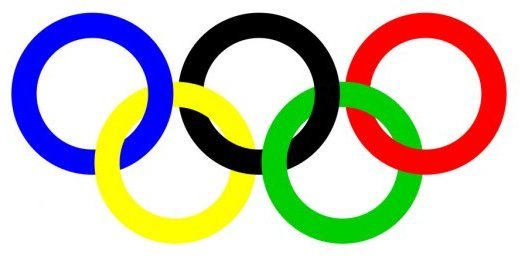
\includegraphics[scale=0.4]{Rings2.jpg}
                \hspace{0.25in}
                
\includegraphics[scale=0.4]{Twitter.jpg}
            \end{figure}

        \subsection{Literature Review}
            Text sentiment analysis is really nothing new. With the advancements of Natural Language Processing (NLP) techniques building a sentiment analysis tool has become commonplace
            in a wide variety of applications. While sentiment analysis is not limited to Twitter and can be used for any text data, with its vast amount of text data and the constant
            addition of data Twitter has been used in many sentiment analysis applications. From using Twitter data to help predict stock data as in 
            \href{http://cs229.stanford.edu/proj2011/GoelMittal-StockMarketPredictionUsingTwitterSentimentAnalysis.pdf}{Anshul Mittal} to the always civil discussions about politics as
            shown in the \href{https://www.geeksforgeeks.org/twitter-sentiment-analysis-using-python/}{Geeks for Geeks article} and 
            \href{https://ieeexplore.ieee.org/abstract/document/6581022?casa_token=qrfkpDZP30sAAAAA:PNpsFf2_T9jXUB81SKLMldZji2tDprsCz4Ec4QSrHxlJQNIW3Yi52tWHZ4jhfTgPrqRjzjdKBfA}{TSAM}. 
            Unsurprisingly, there has been work done in the Olympic domain. The closest work we have discovered documented in a paper was in 
            \href{https://raw.githubusercontent.com/cvorsanger/COMP-4447-Final-Project/master/Literature%20Review/JACET_Volume%205_Issue%203_Page%20143-160.pdf}{2016 Olympic Games on Twitter: Sentiment Analysis of Sports Fans Tweets using Big Data Framework}.
            This paper came out of the Ilamic Azad University in Iran. The writer focuses on Iranian Olympians instead of sports. Using tweets in both English and Farsi they classify
            tweets as fearful, angry, surprising, sadness, joyful, neutral, and anticipation. We will be only concerned about classifying tweets as negative, positive, or neutral.\\

            While most work follows the same general outline there are differences in sentiment analysis works. For instance,
            \href{https://raw.githubusercontent.com/cvorsanger/COMP-4447-Final-Project/master/Literature%20Review/JACET_Volume%205_Issue%203_Page%20143-160.pdf}{2016 Olympic Games on Twitter: Sentiment Analysis of Sports Fans Tweets using Big Data Framework}
            uses the WordNet package to handle most of their preprocessing and sentiment analysis model. 
            \href{https://www.geeksforgeeks.org/twitter-sentiment-analysis-using-python/}{Geeks for Geeks article} uses the TextBlob library for their sentiment analysis. 
            \href{https://towardsdatascience.com/step-by-step-twitter-sentiment-analysis-in-python-d6f650ade58d}{Yalin Yener} introduces the Vader sentiment engine in the nltk library.\\

            After review, we have decided to pursue using mostly the Natural Language ToolKit(NLTK) and the Textblob libraries. With these libraries, we should be able to do most of the
            data cleaning and allows us to use the Vader sentiment engine. More information on Vader will be presented in the Model Creation section.

    \section{Ingestion}
        \subsection{Motivation}
            A particular interest of the authors is the ongoing Summer Olympic games. We enjoy watching the top athletes in the world compete in sports that are not on television very
            often; sports like, gymnastics, swimming, and track. A natural curiosity than was to see how other people view the Olympics. \\

            As social media has grown Twitter has been the go-to platform for the world to express their views. Twitter allows people to express their feelings on just about any subject
            they desire (for better or for worst). It would make sense then to look at Twitter data to model the sentiment around the Olympics. Luckily, Twitter provides an API  for us
            to query historical tweet data.

        \subsection{Ingestion}
            The Twitter API is a relatively easy-to-use API. There are a few restrictions such as rate limits and API types that you do have to consider. For the purposes of this study,
            the API makes it easy to look at historical tweets containing specific words and hashtags. The following details certain aspects of the Twitter API that pertains to this
            project. For more information please visit \href{https://developer.twitter.com/en/docs/twitter-api}{here}. \\

            The first step is to get authorization. To get this we must provide the API with our given client key and secret using the POST command with the requests library. Once we
            get POST we will receive a response from the API we must save.
            
            \begin{lstlisting}[caption=Authorization]
import numpy as np
import pandas as pd
import requests 
import base64

# Save Authorization Info.
client_key = 'XXXXXXXXXXXXXXXXXXXXXXXXXX' 
client_secret = 'XXXXXXXXXXXXXXXXXXXXXXXXXX' 
bearer_token = 'XXXXXXXXXXXXXXXXXXXXXXXXXX' 
key_secret = '{}:{}'.format(client_key, client_secret) \\
    .encode('ascii')
b64_encoded_key = base64.b64encode(key_secret)
b64_encoded_key = b64_encoded_key.decode('ascii')

# Build API URL 
base_url = 'https://api.twitter.com/'
auth_endpoint = base_url + 'oauth2/token'
auth_headers = { 'Authorization': 'Basic {}'  \\
    .format(b64_encoded_key),
                'Content-Type': \\
    'application/x-www-form-urlencoded;charset=UTF-8' }
auth_data = { 'grant_type': 'client_credentials' }

# Provide Authorization Info and Save Access Token
response = requests.post(auth_endpoint, headers=auth_headers, \\
    data=auth_data)
print("Response Status Code: ",response.status_code)
            \end{lstlisting}

            As expected we get a response status code of "200". This tells us that we succesfully recieved our response. The next step is to get the \textit{access token} from our 
            authorization response. \\

            A utility function was then created. This function allows us to use the Twitter API to save tweets. The function needs the user's saved access token and allows for the user
            to specify the number of tweets to pull. The most important parameter of this function is the query parameter. This allows you to filter the tweets you receive by specific
            hashtags, words, retweets, etc. For this project, we are concerned with tweets containing the hashtags "\#olympics" and containing the specific sport. \\

            \begin{lstlisting}[caption=Tweet Generator]
def get_tweets(access_token, query, max_tweets=10, tweet_limit=10):

    page_token = None
    tweet_data = []
    search_headers = {
        'Authorization': 'Bearer {}'.format(access_token),
        'User-Agent': 'v2FullArchiveSearchPython',
    }
    # Divides the max tweets into the appropriate number of 
    # requests based on the tweet_limit.
    for i in range(max_tweets // tweet_limit - 1):
        search_parameters = {
            'query': query,
            'max_results': tweet_limit,
            'tweet.fields': 'lang,created_at,referenced_tweets, \\
                source,conversation_id'
        }
        # If we reach the 2nd page of results, add a next_token 
        #attribute to the search parameters
        if i > 0:
            search_parameters['next_token'] = page_token

        response = requests.get(search_url, headers=search_headers,\\
            params=search_parameters)
        if response.status_code != 200:
            print(f'\tError occurred: Status Code{response. \\
                status_code}: {response.text}')
        else:
            # We need to check for a result count before doing 
            # anything futher; if we have result_count we have data
            if response.json()['meta']['result_count'] > 0:
                tweet_data.extend(response.json()['data'])
                
                # If a 'next_token' exists, then update the page 
                # token to continue pagination through results
                if 'next_token' in response.json()['meta']:
                    page_token = response.json()['meta']['next_token']
            else:
                print(f'\tNo data returned for query!')
                break        
        print(f'\t{len(tweet_data)} total tweets gathered')
        time.sleep(1)
    return tweet_data
            \end{lstlisting}

            Using the above function we can sample retweets having to do with Olympic gymnastics. Notice that we specify the hashtag "\#olympics", the word "gymnastics" and is a retweet
            in the query parameter. Finally, so we do have to keep requesting data from the Twitter API we save the tweets in a pickle file. This way we can use them later in our
            analysis (and Twitter will not get mad at us for rate-limits).\\
            
            Using the "get\_tweets" function we tried to pull 5000 tweets for the sports basketball, biking, diving, gymnastics, skateboarding, surfing, track, and volleyball. This was
            easily done by changing the query parameter to include the name of the sport.

        \subsection{Sample and Explanation}
        Alright we have pulled in some tweets. Now lets have a look at a sample of the tweets.
        \begin{center}
            \begin{tabular}{ |c|c|c|c| }
                \hline
                text snippet & id & created\_at & conversation\_id \\  
                \hline
                \makecell{c\@Shawn\_Shipp\_ Thank You, \\ Simone Biles - Headph...} & 1423371158443941890 & \makecell{2021-08-05 \\ T19:51:43.000Z} & 1423299151215931392 \\
                \hline
                \makecell{Unexpected fun fact: \\ Liu Yang originally wa...} & 1423471713312854017 & \makecell{2021-08-06 \\ T02:31:17.000Z} & 1423471713312854017 \\
                \hline
                \makecell{Rhythmic Gymnastics looks \\ insane. \#Olympics} & 1424213988720717828 & \makecell{2021-08-08 \\ T03:40:50.000Z} & 1424213988720717828 \\
                \hline
                \makecell{\@kpkuehler Thank You, \\ Simone Biles - Headphone...} & 1423796825761456128 & \makecell{2021-08-07 \\ T00:03:10.000Z} & 1423616706413572103 \\
                \hline
                \makecell{\@Simone\_Biles you are \\ a wonderful human being ...} & 1423812938889142273 & \makecell{2021-08-07 \\ T01:07:12.000Z} & 1423812938889142273 \\
                \hline
            \end{tabular}
        \end{center}
        There is a lot of information about tweets that you recieve can recieve from the API. We have narrowed it down to the important ones for this study:
        
        \begin{itemize}
            \item text - The text of the tweet sent out. This will include user handles, hastags, emojis, and any retweet indicators
            \item id - The unique id given to the tweet. This allows for twitter to store tweets.
            \item created\_at - When the tweet was tweeted. Given in UTC time.
            \item conversation\_id - The unique id given to twitter conversations. We can use this id to get all tweets in an conversation.
        \end{itemize}
    \section{Data Cleaning}
        \subsection{Initial Exploration and Cleaning}
            So, now we have tweets regarding the olympic sports of basketball, biking, diving, gymnastics, skateboarding, surfing, track, and volleyball. All of the tweets were collected
            into a single dataframe. This will make it easier for us to clean, look at, and use all of the tweets at once. During this process a new variable was created,
            \textit{sport}. This varibale will track for us the sport that each tweet is talking about and allows us to segment the tweets later when we build our sentiment model. \\
        
            Using the shape function we find that we have 30554 tweets. Now, time to get our hands dirty and clean the data. \\
        
            As with all text data, there is a lot of cleaning that can be done. For this project, we will be concentrating on the removal of certain entities such as URL links and
            hashtags, removal of stopwords, lemmatization, and general NLP text cleaning. After this NLP-specific cleaning, we should be ready to analyze the sentiment of tweets. \\

            Using the below function we were able to use regular expressions to filter the text of our tweets. This function will remove URLs, user handles, hashtags, punctuations, new
            line characters, and numbers that are in the text of the tweet. \\

            \begin{lstlisting}[caption=Regular Expression Cleaner]
import re
def clean_tweet_text(text):
    # Define any custom replacement pattern and join into an 
    #aggregated pattern
    replacements = [
        r'(@[\w]+)',
        r'http[s]?://(?:[a-zA-Z]|[0-9]|[$-_@.&+]|[!*\(\),]|(?:%[0-9\\ 
            a-fA-F][0-9a-fA-F]))+',
        r'(#\w+)',
        r'[\$&+,:;=?@#|\'<>.^*()%!-/]',
        r'\n',
        r'[0-9]+'
    ]
    aggregate_pattern = r'|'.join(replacements)
    # make regex substitutions in one pass
    clean_text = re.sub(aggregate_pattern, '', text) 
    
    # Return the unicode-stripped text in lowercase
    return clean_text.encode(encoding='ascii', errors='ignore')\\
        .decode('ascii').lower()
            \end{lstlisting}

            Stopwords are common words in the English language such as the, an, a, etc. These words are used much in English but convey little meaning. In most NLP applications stop
            words have very little value and only slow down your model due to their high frequency. While these words shouldn't affect our model that much we will still remove them. The
            NLTK library has provides a wide assortment of tools to use for NLP. It even includes a list of stopwords we can use. By iterating over our text and comparing the text to
            the list of stopwords we can remove them for our tweets. \\

            Next, we will lemmatize our tweets. Lemmatization is a process where words are converted to their dictionary forms. For instance, the word "walking" will be analyzed as
            "walk". Lemmatization will ensure that we have proper words. This is the main reason why we chose to lemmatize instead of stemming as the lexicon in Vader works much better
            with real words. The NLTK library has the WordNetLemmatizer built-in. We will the WordNetLemmatizer to handle the lemmatization for us. \\

        \subsection{Type Conversion}
            We needed to change a few data types. Thankfully, the tweet text was already given to us as an object (string). To make our analysis easier we changed the \textit{tweet id}
            and the \textit{conversation ids} of type int from type object. To facilitate the time aspect of our analysis we needed to also covert the \textit{created\_at} variable to
            a datetime object. \\
            
            This leaves us with these variable types, the correct variable types:

            \begin{center}
                \begin{tabular}{|c|c|}
                    \hline
                    id & int32\\
                    \hline
                    created\_at & datetime64[ns, UTC]\\
                    \hline
                    conversation\_id & int32\\
                    \hline
                    text & object\\
                    \hline
                    sport & object\\
                    \hline
                    withheld & object\\
                    \hline
                    clean\_text & object\\
                    \hline
                    clean\_no\_stops & object\\
                    \hline
                    lemma\_text & object\\
                    \hline
                \end{tabular}
            \end{center}
        \subsection{Missing Values}
            Twitter keeps track of everything about a tweet. This is good news to us because the Twitter API rarely gives you missing values. The below plot shows that there are no
            important missing values.

            \begin{figure}[H]
                \centering
                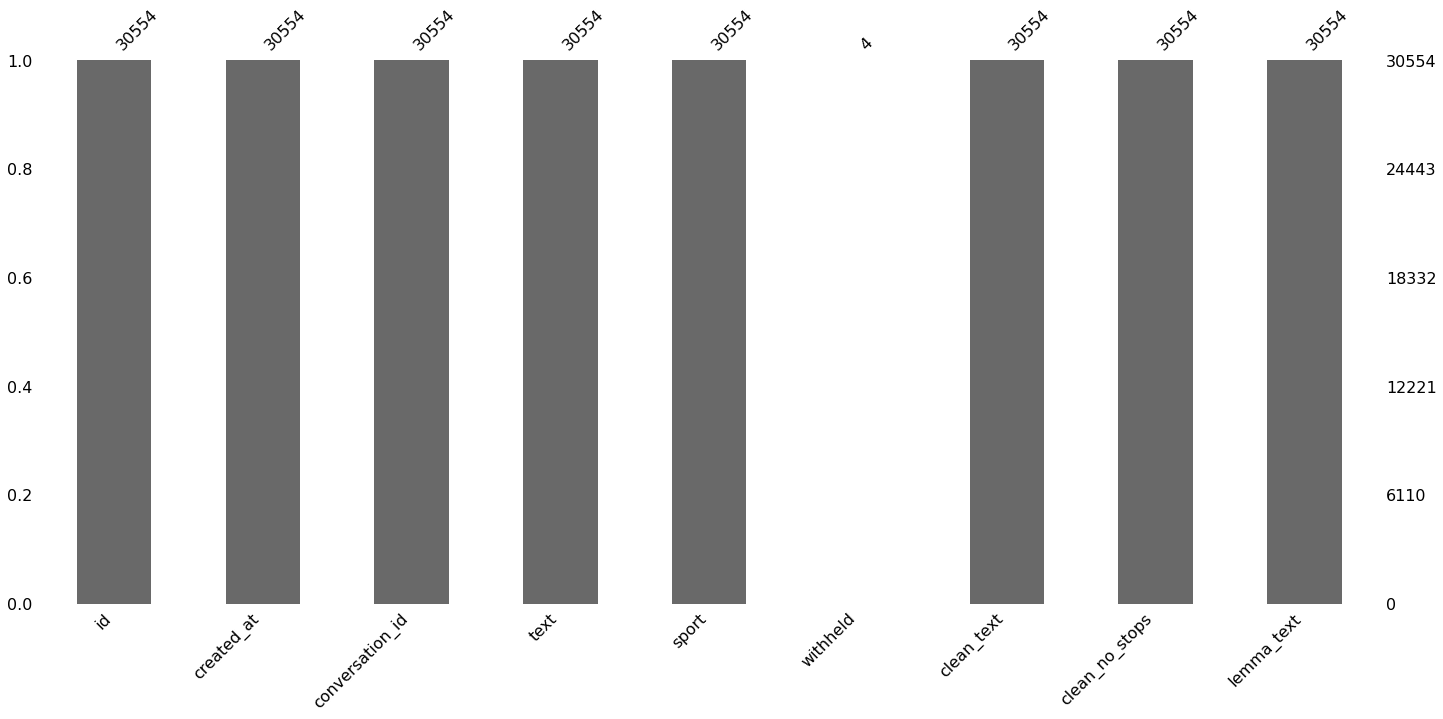
\includegraphics[scale=0.33]{missing.png}
            \end{figure}

            In fact, all of the missing values appear to be in the withheld column. The \textit{withheld} column just tells us in which countries these tweets are not allowed. This is not
            important in analysis and we will therefore just drop that column. \\

            Another precrossing step we can do is to remove an potential dublicates. This was done because dublicate tweet have the potential to skew our data without really telling us 
            anything more.
        \subsection{Outliers}
            With text data, it can be difficult to define what an outlier is. Obviously, be can say obnoxiously positive and negative stuff without really knowing anything; this
            \textit{definitely} doesn't happen on Twitter (wink wink). However, the only real way to detect this is after the sentiment model is built. Also, how do we know what are
            genuine tweets that should be factored in our analysis and bogus tweets that should not? We do assume that most people that are tweeting about the Olympics are at least
            watching them. This is also our main target audience in this study; average people watching the Olympics. With it being impossible to detect bogus tweets from the API and
            our assumption that a vast majority of our tweets originate from our target audience, we decide to analyze all of the tweets we could get. Potentially this could skew our
            sentiment scores. However, we feel confident that with the number of good tweets this potential skew effect should be drowned out.
        \subsection{Additional Exploration}

            \begin{wrapfigure}{l}{0.7\textwidth}
                \centering
                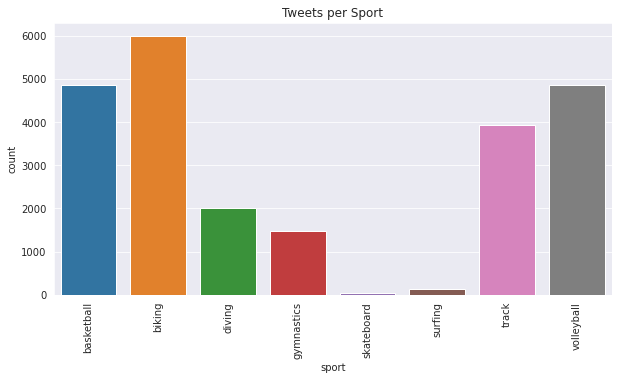
\includegraphics[scale=0.5]{sporttweet.png}
            \end{wrapfigure}

            With text data clean, we can do a little more exploration of the data. \\

            As mentioned earlier we tried to get 5000 tweets for each sport. However, this doesn't guarentee that we will recieve 5000 tweets. With the regular
            twitter API we are limited to tweets created in the past seven days. We did try to upgrade to the acedemic API but were denied, more on the implications 
            of this in \textbf{Section 5.2: Future Work}. Using the \textit{sport} column and the viazualization library seaborn, a histogram was made to convey the number of 
            tweets per sport. \\

            We don't have actually 5000 tweets for any sport! the more popular sports sush as basketball, gymnasticsm track, and volleyball do come close. The newer
            sports such as skateboarding and surfing seem as they are not as talked about. We were surprised by the low number of tweets for diving. While not a 
            super popular sport, diving does seem like it is talked about often when the Summer Olympics come around. Biking does have more tweets then 5000. 
            Initially, we tested our tweets gathering function with a low amount of biking tweets. After we had run our full program we added these initial tweets, 
            which got saved in a pickle file, into the biking tweets pool. Still though, biking appears to be one of the more popular sports. \\

            Wordclouds are another fantastic way to visualize text data. Wordclouds capture the relative frequency of words in a string. The larger the word appears 
            the more frequently it occurs. Words that only appear a couple of times are not pictured in the wordcloud. By concatenating of the tweet text together 
            into one string we can create an overall wordcloud regardless of sport.\\ 

            The phrase "gold medal" appears to be in a ton of tweets as it looms large in the wordcloud. The name of sports in unsurprisinly said alot, as you can 
            see "basketbal", "track", "volleyball",  and "cycling" fairly easily. There are a few athletes that appear in the wordcloud as well. Simone Biles is of 
            course the famous American gymnast. Another name is Anna Kiesenhofer. She is a cyclist that won Austria's first Summer Olympic gold medal since 2004. An 
            interesting word that appears is the word camel. After researching this a little bit, it appears this is in reference to a derogatory term a German 
            cycling coach used in reference to some of the competitors. \\

            \begin{figure}[H]
                \centering
                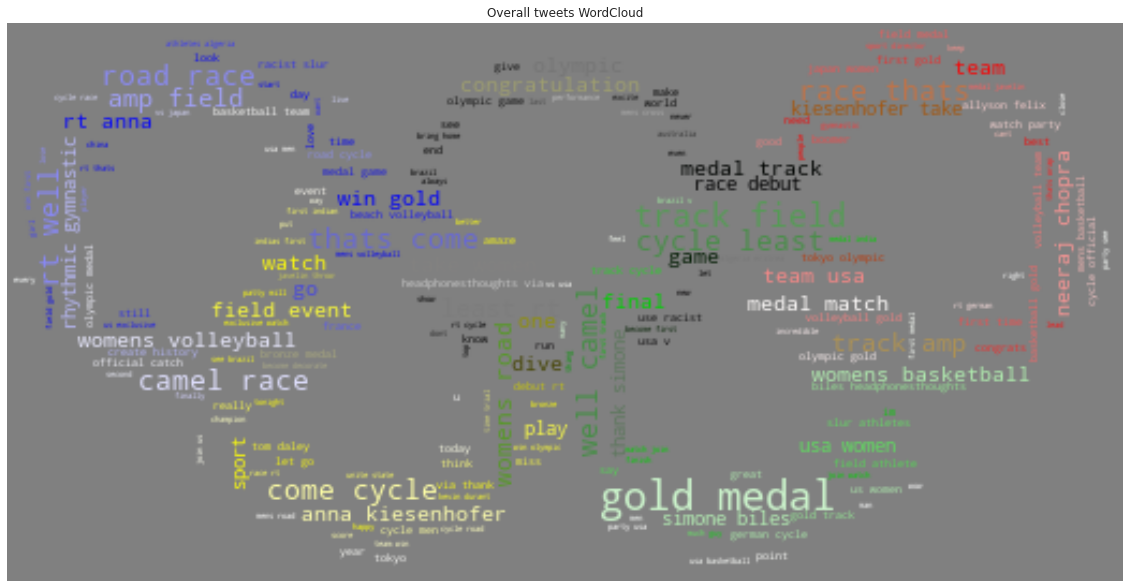
\includegraphics[scale=0.4]{wordcloud.png}
            \end{figure}

            Wordclouds can also be made for each sport.

            \begin{figure}[H]
                \centering
                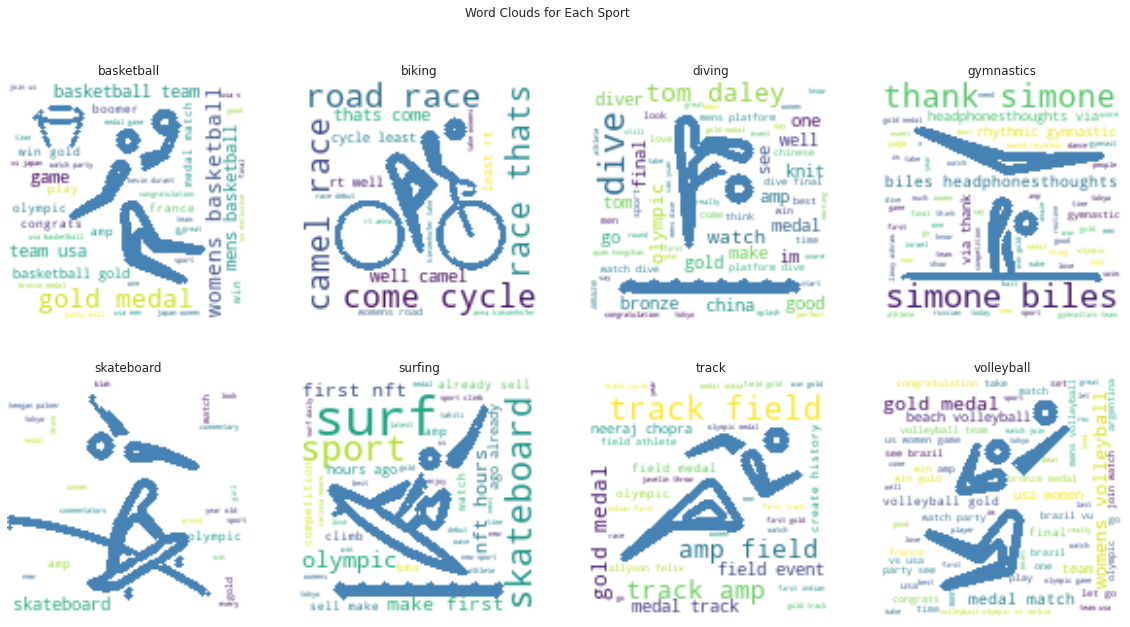
\includegraphics[scale=0.4]{sportsclouds.png}
            \end{figure}

            Noticeably skateboarding has very little words. This is due to the small amount of tweets collected. Skateboarding also appears in the surfing wordcloud. 
            A few of these tweets were reviewed and it appears that surfing and skateboarding were talked about in the same tweet. Simone Biles was very popular in 
            the gymnastics tweets. The british athlete Tom Daley appears in the diving wordcloud.

    \section{Model Creation}
        \subsection{Model}

        To provide sentiment analysis for tweet data, we utilize two packages: (1) TextBlob and (2) VADER from the NLTK toolkit. TextBlob provides a simple interface 
        for processing text-based data and allows for the calculation of the subjectivity and polarity for a given text, which will aid in sentiment analysis using a 
        set of additional text features. The VADER model is a pre-trained model that uses rule-based values which are especially attuned to sentiments from social 
        media, making it a great choice for overall sentiment analysis. \\

        \noindent From the output of TextBlob, we generate two additional features for use in our analysis:
        \begin{itemize}
            \item Polarity: a measure ([-1, 1]) of the sentiment of a text; higher polarity means the text contains more positive sentiment.
            \item Subjectivity: a measure ([0, 1]) of the opinion and factual information contained in a text; higher subjectivity means the text contains more personal opinion.
        \end{itemize}
        
        \noindent From the output of VADER, we generate three additional features for use in our analysis:
        \begin{itemize}
            \item \textit{Neg, Neu,} and \textit{Pos} are scores for the ratios for proportions of text that fall into a negative, neutral, and positive sentiment.
            \item Compound: a score computed by summing the valence scores of each word in the VADER lexicon and normalized to create a composite sentiment score.
            \item Sentiment: a categorical column that standardizes/generalizes the compound score into positive, neutral, and negative sentiment values.
        \end{itemize}
        
        \begin{lstlisting}[caption=Authorization]
# Calculating polarity and subjectivity
olympic_df[['polarity', 'subjectivity']] = olympic_df['lemma_text']\\
    .apply(lambda text: pd.Series(TextBlob(' '.join(text)) \\
    .sentiment))

# Calculating Negative, Positive, Neutral and Compound values
for index, row in olympic_df['clean_no_stops'].iteritems():
    score = SentimentIntensityAnalyzer().polarity_scores(' ' \\
        .join(row))
    neg = score['neg']
    neu = score['neu']
    pos = score['pos']
    comp = score['compound']

    if comp <= -0.05:
        olympic_df.loc[index, 'sentiment'] = 'negative'
    elif comp >= 0.05:
        olympic_df.loc[index, 'sentiment'] = 'positive'
    else:
        olympic_df.loc[index, 'sentiment'] = 'neutral'
    # # Set the values as columns
    olympic_df.loc[index, 'neg'] = neg
    olympic_df.loc[index, 'neu'] = neu
    olympic_df.loc[index, 'pos'] = pos
    olympic_df.loc[index, 'compound'] = comp
        \end{lstlisting}

    \noindent A snippet of our data after running our model will look like:

    \begin{center}
        \begin{tabular}{|c|c|c|c|c|c|c|c|}
            \hline
            lemma\_text & polarity & \makecell{subjec- \\tivity} & sentiment & neg & neu & pos & compound\\
            \hline
            \makecell{[congratulations, tochelsea, \\ grayon, bring, ho...} & 1.000 & 1.000 & positive & 0.0 & 0.456 & 0.544 & 0.9493\\
            \hline
            \makecell{[talkin, noise, podcast, ep, \\ basketball, team,...} & 0.650 & 0.650 & positive & 0.0 & 0.678 & 0.322 & 0.5859\\
            \hline
            \makecell{[high, stake, take, lock, \\ still, day, streak, ...} & 0.144 & 0.513 & positive & 0.0 & 0.865 & 0.135 & 0.4215\\
            \hline
            \makecell{[thursday, qampaclick, \\ link, bio]} & 0.000 & 0.000 & neutral & 0.0 & 1.000 & 0.000 & 0.0000\\
            \hline
            \makecell{[st, three, theme, article, \\ weeks, focus, amaz...} & 0.500 & 0.400 & positive & 0.0 & 0.598 & 0.402 & 0.8555\\
            \hline
        \end{tabular}
    \end{center}

    \section{Evaluation and Conclusions}
        \subsection{Results}
        \begin{wrapfigure}{r}{0.80\textwidth}
            \centering
            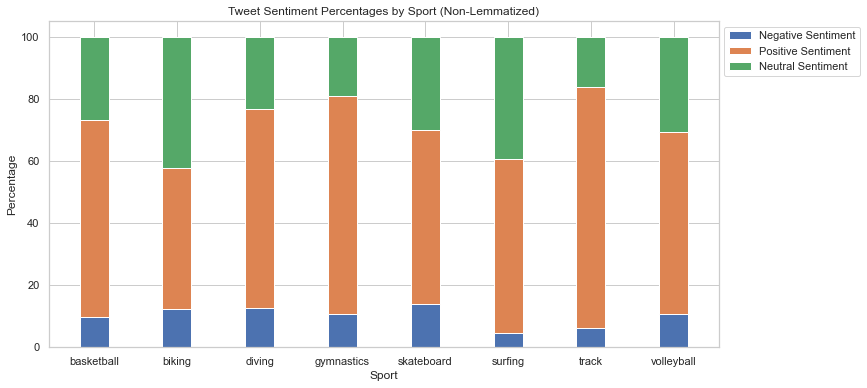
\includegraphics[width=.9\linewidth]{bar.png}
        \end{wrapfigure}
        With all of our tweets scored for sentiment and polarity we can get an idea of the popular sports in the Olympics. A simple bar chart could go along way in drawing our 
        conclusions. \\

        We can also compare sentiment as well as the score differences betweetn Vader and Textblob by a scatter plot. If Vader and Textblob agree completly we should get a 
        diagnoal line from the lower left to the upper right of each scatter plot. 
        \begin{wrapfigure}{l}{0.7\textwidth}
            \centering
            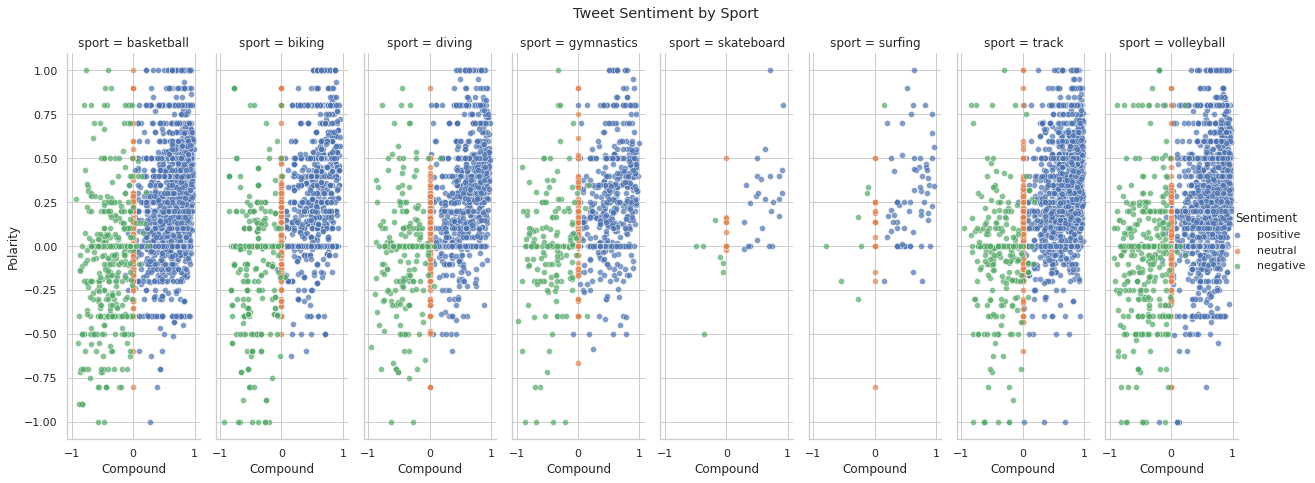
\includegraphics[scale=0.5, angle =-90]{Sentiment.png}
        \end{wrapfigure}

        It appears that all of the sports were talked about in mostly a positive light. The traditional Summer Olympic sports of gymnastics and track were overwelmingly positive with 
        about 70\% of their tweets interpreted as positive. Of the two new sports, skateboarding and surfing, both had slightly positive reactions. Interestingly, out of all of the 
        sports investigated surfing was talked about least neagtively. Biking was the most indifferent sport with just over 40\% of tweets interpreted as neutral tweets. \\

        There does seem to be general agreement between TextBlob and Vader, although it is far from perfect. Both classified more tweets as positive then either neutral or negative. Most 
        points are in the upper right quandrant of their respective scatter plots. This goes back to the two methods generally agreeing. It is clear that not as many tweets for skateboarding 
        or surfing were collected. There were some tweets that the methods completly disagreed on (one said strongly positive and the other said strongly negative). Looking at the two 
        methods combined it would appear that basketball,track, volleyball had the most positive tweets. Biking and diving look as if they have the most neautral tweets. \\

        The fact that most sports were talked about positively was not surprising to us. When the Olympics are on there is generally a positive feel around them. We believe this to be 
        for a few reasons; they are not every year, other then basketball the sports are more niche and not considered to be American major sports, the country vs. country format 
        actually helps breed comradery. We were surprised about the small sample size we were able to collect regarding the two newer sports. While skateboarding and surfing did not 
        seem like they were on mush we anticipated alot more tweets regarding them. \\


        \subsection{Future Work}
        There are several areas where improvements can be made or into which we would invest additional time/resources. A few examples include:

        \begin{itemize}
            \item Exploration and comparison between originating tweet sentiment and tweet reply sentiment to analyze differences
            \item Time-series analysis of sentiment over time for given sport(s)
        \end{itemize}

        One major aspect that could imporve this project as well is type of Twitter API you use. Unfortunatley, we were only able to use the standard API. This had Twitter's lowest rate 
        limit and is restrictive to tweets generated in the last seven days. At the start of this project we did apply to use the Academic API but twitter denied us. The Acedemic API would 
        have been mush more appropiate for this project. With the upgraded API we would have been able to search the full-archive of tweets dating back to 2006 when Twitter started. Also, 
        we would have been able to pull ten million tweets. With a greater breadth of data this project could have been greatly enhanced.

\end{document}